% answers.tex —— 1977 年·青海卷 · 参考答案与详细解析片段
% 由 tools/generate_projects.py 依来源总账自 1977/1977_数学真题_青海_试题.md + 1977/1977_数学真题_青海_解析正文.md + 1977/1977_数学真题_青海_答案要点.md 生成，勿手改（改源 MD 后重跑）


\begin{gktip}
固定源是题面与解答连续出现的《青海1977年高考数学试题解》扫描材料（第 1—4 页）。下文逐题独立推导，并对照源解答复算关键结论。第 4 题源卷子项编号“1．”“2．”已重排为（1）（2）；第五题四次根号内 $b$ 的指数按 600dpi 局部放大目视并结合源解答中间步骤判定为 $b^{\frac43}$（见试题第 5 题源注）。
\end{gktip}

\begin{answer}
\gksolhead{1}{}

\textbf{题目}：

\Needspace{5\baselineskip}
计算：

\nopagebreak[4]
\[
\frac{a}{a-b}-\frac{b}{a+b}+\frac{2ab}{a^2-b^2}\cdot(a\ne\pm b).
\]

\Needspace{4\baselineskip}
\textbf{解析}

\Needspace{5\baselineskip}
$a\ne\pm b$ 保证各分母非零。通分：

\nopagebreak[4]
\[
\frac{a}{a-b}-\frac{b}{a+b}+\frac{2ab}{(a-b)(a+b)}
=\frac{a(a+b)-b(a-b)+2ab}{(a-b)(a+b)}.
\]

\Needspace{5\baselineskip}
分子

\nopagebreak[4]
\[
a(a+b)-b(a-b)+2ab=a^2+ab-ab+b^2+2ab=a^2+b^2+2ab=(a+b)^2.
\]

\Needspace{5\baselineskip}
约去非零因式 $a+b$：

\nopagebreak[4]
\[
\text{\text{原式}}=\frac{(a+b)^2}{(a-b)(a+b)}=\frac{a+b}{a-b}.
\]

\gkanswer{答案：$\dfrac{a+b}{a-b}$。}

\end{answer}
\begin{answer}
\gksolhead{2}{}

\textbf{题目}：

如图，$AB$ 是 $\odot O$ 的直径，$AC$ 是 $\odot O$ 的切线，连接 $BC$ 与 $\odot O$ 相交于 $D$ 点，而且 $\angle ABC=45^\circ$。求证 $BD=DC$。

\begin{gktip}
原源 PDF 第 1 页附有圆、切线与弦的示意图；LaTeX 版按源图重绘。
\end{gktip}
\nopagebreak[4]
\begin{center}% 1977 年青海卷第二题：圆 O、直径 AB（水平）、切线 AC（A 处竖直）、弦 CB 交圆于 D，
% 辅助线 AD 为虚线，∠ABC=45° 标在 B 处（按源卷第 1 页布局）
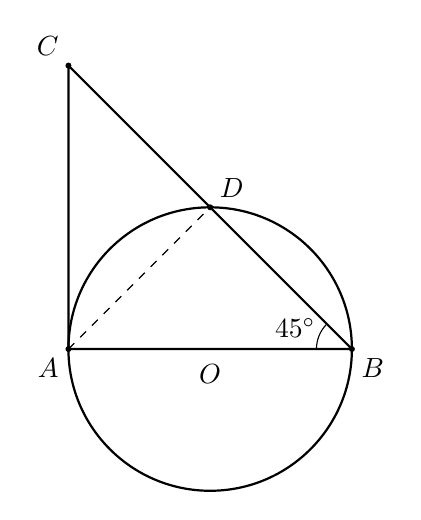
\begin{tikzpicture}[scale=0.9]
  \draw[thick] (0,0) circle (2);
  \coordinate (A) at (-2,0);
  \coordinate (B) at (2,0);
  \coordinate (C) at (-2,4);
  \coordinate (D) at (0,2);
  \draw[thick] (A)--(C)--(B)--cycle;
  \draw[dashed] (A)--(D);
  \fill (A) circle (1.2pt) node[below left] {$A$};
  \fill (B) circle (1.2pt) node[below right] {$B$};
  \fill (C) circle (1.2pt) node[above left] {$C$};
  \fill (D) circle (1.2pt) node[above right] {$D$};
  \node at (0,-0.35) {$O$};
  \draw ([shift={(180:0.5)}]B) arc[start angle=180, end angle=135, radius=0.5];
  \node at (1.2,0.3) {$45^\circ$};
\end{tikzpicture}
\end{center}
\nopagebreak[4]
\Needspace{4\baselineskip}
\textbf{解析}

连接 $AD$。

\Needspace{5\baselineskip}
$AB$ 是直径，故 $\angle ADB=90^\circ$（直径所对的圆周角）。在 $\triangle ABD$ 中 $\angle ABD=45^\circ$，所以 $\angle BAD=45^\circ$，从而

\nopagebreak[4]
\[
BD=AD.
\]

\Needspace{5\baselineskip}
$AC$ 是 $\odot O$ 的切线而 $AB$ 为直径，故 $AC\perp AB$，即 $\angle BAC=90^\circ$，于是

\nopagebreak[4]
\[
\angle DAC=90^\circ-45^\circ=45^\circ.
\]

\Needspace{5\baselineskip}
因 $B\text{、}D\text{、}C$ 三点共线，$\angle ADC=180^\circ-\angle ADB=90^\circ$。在 $\mathrm{Rt}\triangle ACD$ 中 $\angle DAC=45^\circ$，故 $\angle ACD=45^\circ$，从而

\nopagebreak[4]
\[
DC=AD.
\]

所以 $BD=DC$。
\nopagebreak[4]
\begin{center}% 1977 年青海卷第二题：圆 O、直径 AB（水平）、切线 AC（A 处竖直）、弦 CB 交圆于 D，
% 辅助线 AD 为虚线，∠ABC=45° 标在 B 处（按源卷第 1 页布局）
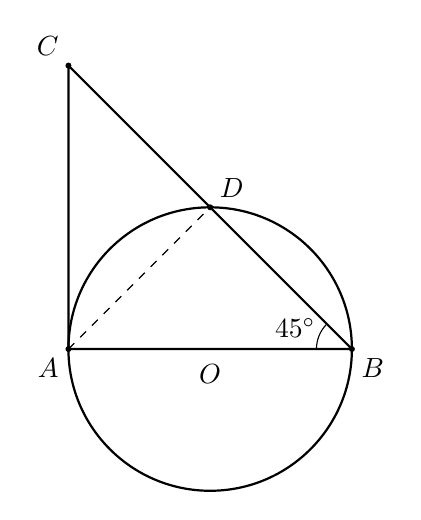
\begin{tikzpicture}[scale=0.9]
  \draw[thick] (0,0) circle (2);
  \coordinate (A) at (-2,0);
  \coordinate (B) at (2,0);
  \coordinate (C) at (-2,4);
  \coordinate (D) at (0,2);
  \draw[thick] (A)--(C)--(B)--cycle;
  \draw[dashed] (A)--(D);
  \fill (A) circle (1.2pt) node[below left] {$A$};
  \fill (B) circle (1.2pt) node[below right] {$B$};
  \fill (C) circle (1.2pt) node[above left] {$C$};
  \fill (D) circle (1.2pt) node[above right] {$D$};
  \node at (0,-0.35) {$O$};
  \draw ([shift={(180:0.5)}]B) arc[start angle=180, end angle=135, radius=0.5];
  \node at (1.2,0.3) {$45^\circ$};
\end{tikzpicture}
\end{center}
\nopagebreak[4]
\gkanswer{答案：见解析版}

\end{answer}
\begin{answer}
\gksolhead{3}{}

\textbf{题目}：

已知长方体 $ABCD\text{-}A'B'C'D'$ 的对角线 $AC'$ 与 $A'C$ 的夹角 $\angle AOC=120^\circ$，底面边长 $AB=4\,\mathrm{cm}$，$BC=3\,\mathrm{cm}$。求此长方体的体积。

\begin{gktip}
\textbf{源注}：原卷印作“$\angle AoC=120^\circ$”“$AB=4Cm$”（字母大小写排印不一致），本库按规范记法转录。
原源 PDF 第 1 页附有长方体及体对角线夹角示意图；LaTeX 版按源图重绘。
\end{gktip}
\nopagebreak[4]
\begin{center}% 1977 年青海卷第三题：长方体 ABCD-A'B'C'D'（顶面 A'B'C'D'），底面 ABCD（A 前左、B 前右、
% C 后右、D 后左），体对角线 AC' 与 A'C 交于体心 O，∠AOC=120°，辅助线底面对角线 AC（虚线）
%（按源卷第 1 页布局）
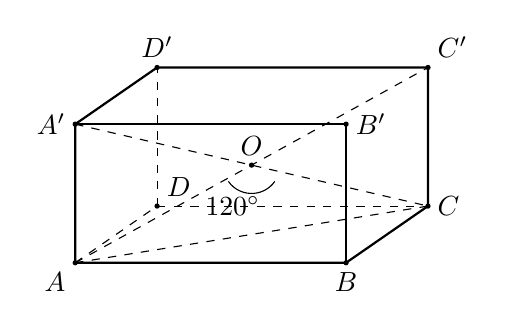
\begin{tikzpicture}[scale=0.8]
  \coordinate (A) at (0,0);
  \coordinate (B) at (4.3,0);
  \coordinate (C) at (5.6,0.9);
  \coordinate (D) at (1.3,0.9);
  \coordinate (A1) at (0,2.2);
  \coordinate (B1) at (4.3,2.2);
  \coordinate (C1) at (5.6,3.1);
  \coordinate (D1) at (1.3,3.1);
  \coordinate (O) at (2.8,1.55);
  \draw[thick] (A)--(B)--(C)--(C1)--(D1)--(A1)--cycle;
  \draw[thick] (A)--(A1);
  \draw[thick] (B)--(B1);
  \draw[thick] (A1)--(B1);
  \draw[dashed] (A)--(D);
  \draw[dashed] (D)--(C);
  \draw[dashed] (D)--(D1);
  \draw[dashed] (A)--(C);
  \draw[dashed] (A)--(C1);
  \draw[dashed] (A1)--(C);
  \fill (A) circle (1.2pt) node[below left] {$A$};
  \fill (B) circle (1.2pt) node[below] {$B$};
  \fill (C) circle (1.2pt) node[right] {$C$};
  \fill (D) circle (1.2pt) node[above right] {$D$};
  \fill (A1) circle (1.2pt) node[left] {$A'$};
  \fill (B1) circle (1.2pt) node[right] {$B'$};
  \fill (C1) circle (1.2pt) node[above right] {$C'$};
  \fill (D1) circle (1.2pt) node[above] {$D'$};
  \fill (O) circle (1.2pt) node[above] {$O$};
  \draw ([shift={(215:0.45)}]O) arc[start angle=215, end angle=325, radius=0.45];
  \node at (2.5,0.9) {$120^\circ$};
\end{tikzpicture}
\end{center}
\nopagebreak[4]
\Needspace{4\baselineskip}
\textbf{解析}

\Needspace{5\baselineskip}
长方体中心对称，体对角线 $AC'$ 与 $A'C$ 互相平分于体心 $O$，故 $CO=C'O$，且 $A\text{、}O\text{、}C'$ 共线。由 $\angle AOC=120^\circ$ 得

\nopagebreak[4]
\[
\angle COC'=180^\circ-120^\circ=60^\circ.
\]

\Needspace{5\baselineskip}
$\triangle COC'$ 等腰且顶角为 $60^\circ$，故底角

\nopagebreak[4]
\[
\angle OCC'=\angle OC'C=60^\circ.
\]

\Needspace{5\baselineskip}
连接 $AC$。侧棱 $CC'\perp$ 底面 $ABCD$，故 $CC'\perp AC$，$\triangle ACC'$ 为直角三角形（直角在 $C$）。因 $C'$ 在直线 $CO$ 上，$\angle AC'C=\angle OC'C=60^\circ$，于是

\nopagebreak[4]
\[
\angle C'AC=90^\circ-60^\circ=30^\circ.
\]

\Needspace{5\baselineskip}
直角三角形中 $30^\circ$ 角所对的直角边等于斜边的一半：

\nopagebreak[4]
\[
AC'=2C'C.
\]

\Needspace{5\baselineskip}
底面矩形对角线

\nopagebreak[4]
\[
AC=\sqrt{AB^2+BC^2}=\sqrt{4^2+3^2}=5.
\]

\Needspace{5\baselineskip}
设 $C'C=x$，则 $AC'=2x$。在 $\mathrm{Rt}\triangle ACC'$ 中用勾股定理：

\nopagebreak[4]
\[
(2x)^2=5^2+x^2
\quad\Longrightarrow\quad
3x^2=25
\quad\Longrightarrow\quad
x=\frac{5\sqrt3}{3}.
\]

\Needspace{5\baselineskip}
所以长方体体积

\nopagebreak[4]
\[
V=AB\times BC\times C'C=4\times3\times\frac{5\sqrt3}{3}=20\sqrt3\ (\mathrm{cm^3}).
\]
\nopagebreak[4]
\begin{center}% 1977 年青海卷第三题：长方体 ABCD-A'B'C'D'（顶面 A'B'C'D'），底面 ABCD（A 前左、B 前右、
% C 后右、D 后左），体对角线 AC' 与 A'C 交于体心 O，∠AOC=120°，辅助线底面对角线 AC（虚线）
%（按源卷第 1 页布局）
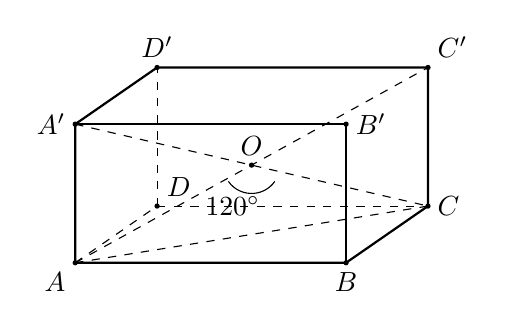
\begin{tikzpicture}[scale=0.8]
  \coordinate (A) at (0,0);
  \coordinate (B) at (4.3,0);
  \coordinate (C) at (5.6,0.9);
  \coordinate (D) at (1.3,0.9);
  \coordinate (A1) at (0,2.2);
  \coordinate (B1) at (4.3,2.2);
  \coordinate (C1) at (5.6,3.1);
  \coordinate (D1) at (1.3,3.1);
  \coordinate (O) at (2.8,1.55);
  \draw[thick] (A)--(B)--(C)--(C1)--(D1)--(A1)--cycle;
  \draw[thick] (A)--(A1);
  \draw[thick] (B)--(B1);
  \draw[thick] (A1)--(B1);
  \draw[dashed] (A)--(D);
  \draw[dashed] (D)--(C);
  \draw[dashed] (D)--(D1);
  \draw[dashed] (A)--(C);
  \draw[dashed] (A)--(C1);
  \draw[dashed] (A1)--(C);
  \fill (A) circle (1.2pt) node[below left] {$A$};
  \fill (B) circle (1.2pt) node[below] {$B$};
  \fill (C) circle (1.2pt) node[right] {$C$};
  \fill (D) circle (1.2pt) node[above right] {$D$};
  \fill (A1) circle (1.2pt) node[left] {$A'$};
  \fill (B1) circle (1.2pt) node[right] {$B'$};
  \fill (C1) circle (1.2pt) node[above right] {$C'$};
  \fill (D1) circle (1.2pt) node[above] {$D'$};
  \fill (O) circle (1.2pt) node[above] {$O$};
  \draw ([shift={(215:0.45)}]O) arc[start angle=215, end angle=325, radius=0.45];
  \node at (2.5,0.9) {$120^\circ$};
\end{tikzpicture}
\end{center}
\nopagebreak[4]
\gkanswer{答案：$20\sqrt3\ \mathrm{cm^3}$。}

\end{answer}
\begin{answer}
\gksolhead{4}{}

\textbf{题目}：

求下列函数的定义域：

（1） $y=\dfrac{7x}{x+1}$

（2） $y=\dfrac{1}{\sqrt{2-x}}$

\begin{gktip}
\textbf{题号说明}：原卷两个子项编号为“1．”“2．”，本库按小问格式重排为（1）（2），未增删内容。
\end{gktip}

\Needspace{4\baselineskip}
\textbf{解析}

\gksubpart{（1）}

分式有意义要求分母 $x+1\ne0$，即 $x\ne-1$。定义域为 $x$ 不等于 $-1$ 的任意实数。

\gksubpart{（2）}

偶次根号下被开方数非负且分母非零，要求 $2-x>0$，即 $x<2$。定义域为 $x<2$ 的实数。

\gkanswer{答案（1）：$x\ne-1$ 的任意实数。}

\gkanswer{答案（2）：$x<2$ 的实数。}

\end{answer}
\begin{answer}
\gksolhead{5}{}

\textbf{题目}：

化简：

\begin{gktip}
\textbf{源注}：四次根号内 $b$ 的指数在扫描件中不易分辨，按 600dpi 局部放大目视为 $b^{\frac43}$（无负号），并与源解答中间步骤 $(ab^{-\frac13}\cdot b^{\frac13})^{\frac12}$ 及化简结果 $3a$ 交叉一致。
\end{gktip}

\nopagebreak[4]
\[
\left(27a^{\frac52}\sqrt{ab^{-\frac13}\sqrt[4]{b^{\frac43}}}\right)^{\frac13}\qquad(b\ne0).
\]

\Needspace{4\baselineskip}
\textbf{解析}

\Needspace{5\baselineskip}
条件 $b\ne0$ 保证各负指数幂有意义。先算四次根：

\nopagebreak[4]
\[
\sqrt[4]{b^{\frac43}}=b^{\frac{4}{3}\cdot\frac14}=b^{\frac13}.
\]

\Needspace{5\baselineskip}
代入大根号内：

\nopagebreak[4]
\[
ab^{-\frac13}\cdot b^{\frac13}=a,
\]

\Needspace{5\baselineskip}
所以外层平方根为 $\sqrt a=a^{\frac12}$。原式

\nopagebreak[4]
\[
\left(27a^{\frac52}\cdot a^{\frac12}\right)^{\frac13}
=\left(27a^3\right)^{\frac13}
=3a.
\]

\gkanswer{答案：$3a$。}

\end{answer}
\begin{answer}
\gksolhead{6}{}

\textbf{题目}：

计算：$\lg14-2\lg\dfrac73+\lg7-\lg18$

\Needspace{4\baselineskip}
\textbf{解析}

\Needspace{5\baselineskip}
利用 $\lg14=\lg2+\lg7$、$2\lg\dfrac73=2(\lg7-\lg3)$、$\lg18=2\lg3+\lg2$：

\nopagebreak[4]
\[
\text{\text{原式}}=(\lg2+\lg7)-2(\lg7-\lg3)+\lg7-(2\lg3+\lg2)=0.
\]

也可合并为一个对数验证：$\dfrac{14\times7}{\left(\frac73\right)^2\times18}=\dfrac{98}{98}=1$，故原式 $=\lg1=0$。

\gkanswer{答案：$0$。}

\end{answer}
\begin{answer}
\gksolhead{7}{}

\textbf{题目}：

求 $\sin435^\circ$ 的值。

\Needspace{4\baselineskip}
\textbf{解析}

\nopagebreak[4]
\[
\sin435^\circ=\sin(360^\circ+75^\circ)=\sin75^\circ=\sin(45^\circ+30^\circ).
\]

\Needspace{5\baselineskip}
用两角和公式：

\nopagebreak[4]
\[
\sin75^\circ=\sin45^\circ\cos30^\circ+\cos45^\circ\sin30^\circ
=\frac{\sqrt2}{2}\cdot\frac{\sqrt3}{2}+\frac{\sqrt2}{2}\cdot\frac12
=\frac{\sqrt6+\sqrt2}{4}.
\]

\gkanswer{答案：$\dfrac{\sqrt6+\sqrt2}{4}$。}

\end{answer}
\begin{answer}
\gksolhead{8}{}

\textbf{题目}：

\Needspace{5\baselineskip}
当锐角 $\theta$ 为何值时，方程

\nopagebreak[4]
\[
(3\sin\theta)x^2-(4\cos\theta)x+2=0
\]

有两个相等的实数根？并求出这个方程的实数根。

\Needspace{4\baselineskip}
\textbf{解析}

\Needspace{5\baselineskip}
方程 $(3\sin\theta)x^2-(4\cos\theta)x+2=0$ 有两个相等实数根的条件是判别式为零：

\nopagebreak[4]
\[
\Delta=(4\cos\theta)^2-4\cdot(3\sin\theta)\cdot2=16\cos^2\theta-24\sin\theta=0,
\]

\Needspace{5\baselineskip}
即 $2\cos^2\theta-3\sin\theta=0$。用 $\cos^2\theta=1-\sin^2\theta$：

\nopagebreak[4]
\[
2(1-\sin^2\theta)-3\sin\theta=0
\quad\Longrightarrow\quad
2\sin^2\theta+3\sin\theta-2=0,
\]

\Needspace{5\baselineskip}
因式分解：

\nopagebreak[4]
\[
(2\sin\theta-1)(\sin\theta+2)=0
\quad\Longrightarrow\quad
\sin\theta=\frac12\ \text{\text{或}}\ \sin\theta=-2.
\]

后者越出 $|\sin\theta|\le1$，舍去。$\theta$ 为锐角，故 $\theta=30^\circ$。

\Needspace{5\baselineskip}
此时方程为 $\dfrac32x^2-2\sqrt3\,x+2=0$，两边乘 $2$：

\nopagebreak[4]
\[
3x^2-4\sqrt3\,x+4=0
\quad\Longleftrightarrow\quad
(\sqrt3\,x-2)^2=0,
\]

\Needspace{5\baselineskip}
所以方程的两个相等实数根为

\nopagebreak[4]
\[
x=\frac{2}{\sqrt3}=\frac{2\sqrt3}{3}.
\]

\gkanswer{答案：$\theta=30^\circ$；方程的两个相等实数根为 $x=\dfrac{2\sqrt3}{3}$。}

\end{answer}
\begin{answer}
\gksolhead{9}{}

\textbf{题目}：

求经过抛物线 $y^2=-2x$ 的焦点，且与直线 $2x-y-1=0$ 垂直的直线方程。

\Needspace{4\baselineskip}
\textbf{解析}

\Needspace{5\baselineskip}
$y^2=-2x$ 即 $2p=-2$，抛物线开口向左，焦点在 $x$ 轴负半轴：

\nopagebreak[4]
\[
F=\left(\frac{p}{2},0\right)=\left(-\frac12,0\right).
\]

\Needspace{5\baselineskip}
直线 $2x-y-1=0$ 即 $y=2x-1$，斜率为 $2$，所求直线与其垂直，斜率为 $-\dfrac12$。由点斜式，过 $\left(-\dfrac12,0\right)$ 的直线为

\nopagebreak[4]
\[
y-0=-\frac12\left(x+\frac12\right),
\]

\Needspace{5\baselineskip}
整理得

\nopagebreak[4]
\[
2x+4y+1=0.
\]

\gkanswer{答案：$2x+4y+1=0$。}

\end{answer}
\begin{answer}
\gksolhead{10}{}

\textbf{题目}：

今年，我省香日德农场春小麦亩产达 1765.5 斤，创全国春小麦亩产新记录，在大治之年作出了贡献。我省在 1971 年开始出现亩产 1000 斤的高产田。从 1971 年的高产量 1000 斤到今年的创记录产量 1765.5 斤，平均每年的增长率是多少？

（已知 $\lg1.766=0.2470$，已知由 $\lg A=0.0412$ 得 $A=1.100$）

\Needspace{5\baselineskip}
\textbf{参考题 1．} 若齐次线性方程组

\nopagebreak[4]
\[
\begin{cases}
x+ay+a^2z=0\\
ax+a^2y+z=0\\
a^2x+y+az=0
\end{cases}
\]

有非零解，那末 $a$ 应为何值？

\textbf{参考题 2．} 试求由曲线 $y=2\cos x$ 之一半被与 $y=0$ 围成的面积绕 $Ox$ 轴旋转所产生的立体的体积。

\Needspace{4\baselineskip}
\textbf{解析}

\Needspace{5\baselineskip}
从 1971 年到今年共经过 $6$ 年。设平均年增长率为 $x$，则

\nopagebreak[4]
\[
1000(1+x)^6=1765.5
\quad\Longrightarrow\quad
(1+x)^6=1.7655\approx1.766.
\]

\Needspace{5\baselineskip}
两边取常用对数：

\nopagebreak[4]
\[
6\lg(1+x)=\lg1.766=0.2470
\quad\Longrightarrow\quad
\lg(1+x)=\frac{0.2470}{6}\approx0.0412.
\]

\Needspace{5\baselineskip}
由已知 $\lg A=0.0412$ 时 $A=1.100$，故

\nopagebreak[4]
\[
1+x=1.100
\quad\Longrightarrow\quad
x=0.100\approx10.0\%.
\]

即平均每年的增长率约为 $10.0\%$。

\textbf{参考题 1}

\Needspace{5\baselineskip}
齐次线性方程组有非零解的充要条件是系数行列式等于零：

\nopagebreak[4]
\[
\begin{vmatrix}
1 & a & a^2\\
a & a^2 & 1\\
a^2 & 1 & a
\end{vmatrix}=0.
\]

\Needspace{5\baselineskip}
按对角线法则展开：

\nopagebreak[4]
\[
1\cdot a^2\cdot a+a\cdot1\cdot a^2+a^2\cdot a\cdot1
-a^2\cdot a^2\cdot a^2-a\cdot a\cdot a-1\cdot1\cdot1
=3a^3-a^6-1-a^3=2a^3-a^6-1.
\]

\Needspace{5\baselineskip}
所以

\nopagebreak[4]
\[
2a^3-a^6-1=0
\quad\Longleftrightarrow\quad
-(a^6-2a^3+1)=0
\quad\Longleftrightarrow\quad
(a^3-1)^2=0,
\]

故 $a^3=1$，实数解为 $a=1$。即 $a=1$ 时该齐次线性方程组有非零解。

\textbf{参考题 2}

\Needspace{5\baselineskip}
曲线 $y=2\cos x$ 在 $\left[-\dfrac{\pi}{2},\dfrac{\pi}{2}\right]$ 上的一段位于 $x$ 轴上方，它与 $y=0$ 围成的图形绕 $Ox$ 轴旋转一周，所得立体的体积为

\nopagebreak[4]
\[
V=\pi\int_{-\frac{\pi}{2}}^{\frac{\pi}{2}}y^2\,dx
=\pi\int_{-\frac{\pi}{2}}^{\frac{\pi}{2}}4\cos^2x\,dx
=2\pi\int_{-\frac{\pi}{2}}^{\frac{\pi}{2}}(1+\cos2x)\,dx
\]

\nopagebreak[4]
\[
=2\pi\left[x+\frac{\sin2x}{2}\right]_{-\frac{\pi}{2}}^{\frac{\pi}{2}}
=2\pi(\pi+0)=2\pi^2.
\]

\gkanswer{答案：平均年增长率约为 $10.0\%$。}

\end{answer}